% begin module rolles-theorem
\begin{frame}[t]
\begin{theorem}[Rolle's Theorem]
Let $f$ be a function that satisfies the following three conditions:
\begin{itemize}
\item  $f$ is continuous on the closed interval $[a,b]$.
\item  $f$ is differentiable on the open interval $(a,b)$.
\item  $f(a) = f(b)$.
\end{itemize}
Then there is a number $c$ in $(a,b)$ such that $f'(c) = 0$.
\end{theorem}
\begin{columns}[c]
\column{.3\textwidth}
\uncover<3->{%
\ \only<handout:1| -3>{%
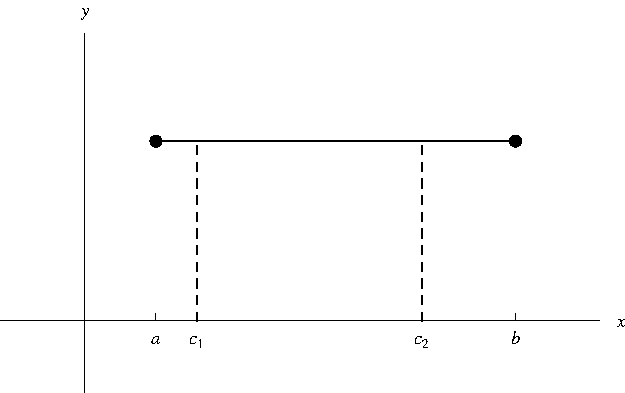
\includegraphics[height=2.2cm]{maxima-minima/pictures/04-02-rollesa.pdf}%
}%
}%
\only<handout:2-3| 4->{%
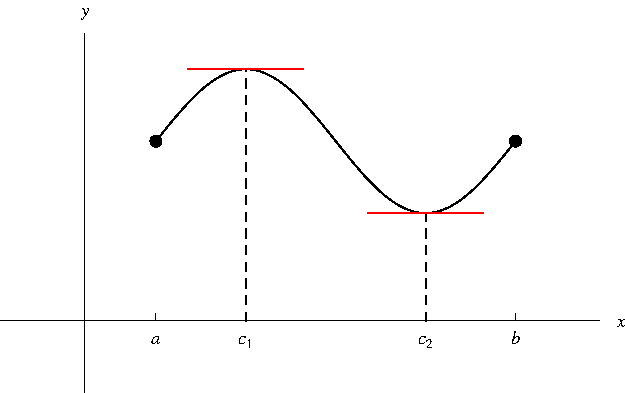
\includegraphics[height=2.2cm]{maxima-minima/pictures/04-02-rollesc.pdf}%
}%

\uncover<handout:2| 4->{%
\ \only<handout:-2| -4>{%
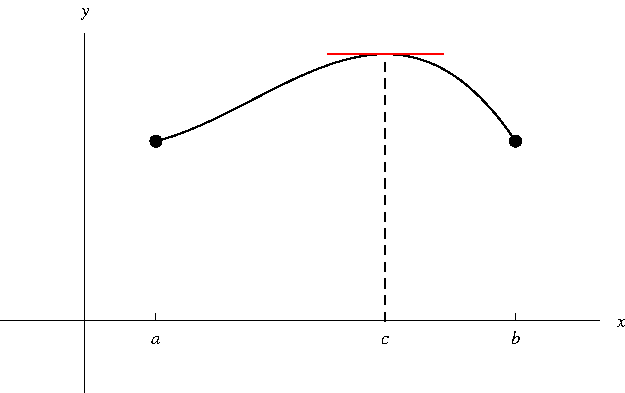
\includegraphics[height=2.2cm]{maxima-minima/pictures/04-02-rollesb.pdf}%
}%
}%
\only<handout:3| 5->{%
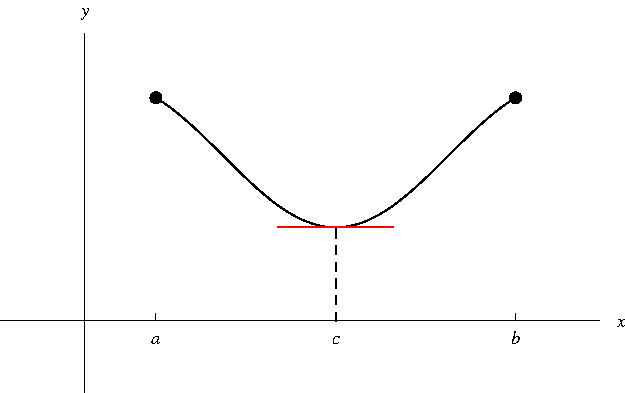
\includegraphics[height=2.2cm]{maxima-minima/pictures/04-02-rollesd.pdf}%
}%
\column{.6\textwidth}
\uncover<2->{%
The proof breaks down into three cases:
\begin{enumerate}
\item<1-| alert@3>  \alert<handout:1| 0>{$f$ is a horizontal line.}
\item<1-| alert@4>  \alert<handout:2| 0>{$f(x) > f(a)$ for some $x$ in $(a,b)$.}
\item<1-| alert@5>  \alert<handout:3| 0>{$f(x) < f(a)$ for some $x$ in $(a,b)$.}
\end{enumerate}
}%
\end{columns}
\end{frame}


\begin{frame}[t]
\begin{theorem}[Rolle's Theorem]
Let $f$ be a function that satisfies the following three conditions:
\begin{itemize}
\item  $f$ is continuous on the closed interval $[a,b]$.
\item  $f$ is differentiable on the open interval $(a,b)$.
\item  $f(a) = f(b)$.
\end{itemize}
Then there is a number $c$ in $(a,b)$ such that $f'(c) = 0$.
\end{theorem}
\begin{proof}
\begin{columns}[c]
\column{.3\textwidth}
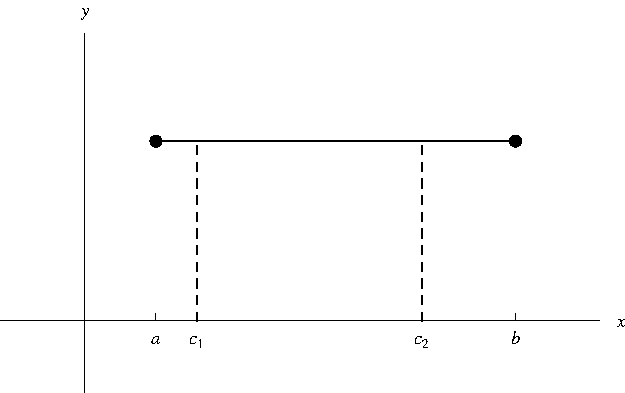
\includegraphics[height=2.5cm]{maxima-minima/pictures/04-02-rollesa.pdf}%
\column{.6\textwidth}
\begin{enumerate}
\item  $f$ is a horizontal line.
\end{enumerate}
\begin{itemize}
\item<2->  Then \alert<handout:0| 2-3>{$f'(x) = \uncover<3->{0.}$}
\item<4->  Therefore we can take $c$ to be any number in $(a,b)$. \qedhere
\end{itemize}
\end{columns}
\end{proof}
\end{frame}


\begin{frame}[t]
\begin{theorem}[Rolle's Theorem]
Let $f$ be a function that satisfies the following three conditions:
\begin{itemize}
\item  $f$ is continuous on the closed interval $[a,b]$.
\item<1-| alert@4>  $f$ is differentiable on the open interval $(a,b)$.
\item<1-| alert@3>  $f(a) = f(b)$.
\end{itemize}
Then there is a number $c$ in $(a,b)$ such that $f'(c) = 0$.
\end{theorem}
\begin{proof}
\begin{columns}[c]
\column{.3\textwidth}
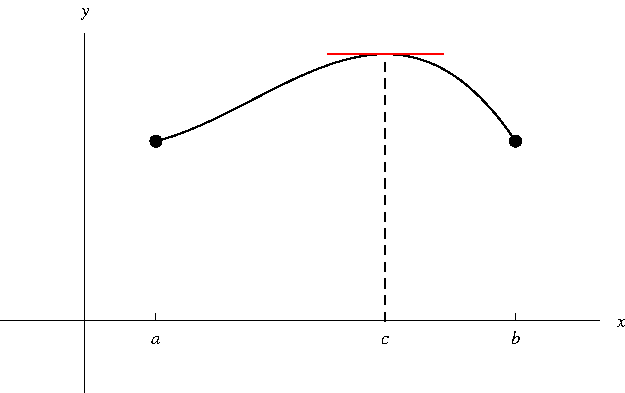
\includegraphics[height=2.5cm]{maxima-minima/pictures/04-02-rollesb.pdf}%
\column{.6\textwidth}
\begin{enumerate}
\setcounter{enumi}{1}
\item  $f(x) > f(a)$ for some $x$ in $(a,b)$.
\end{enumerate}
\begin{itemize}
\item<2->  By the Extreme Value Theorem, $f$ has a maximum in $[a,b]$.
\item<3->  Since $f(x) > f(a)$, this value is attained at some $c$ in $(a,b)$.
\item<4->  \alert<handout:0| 4>{Fermat's Theorem}: $f'(c) = 0$.\qedhere
\end{itemize}
\end{columns}
\end{proof}
\end{frame}



\begin{frame}[t]
\begin{theorem}[Rolle's Theorem]
Let $f$ be a function that satisfies the following three conditions:
\begin{itemize}
\item  $f$ is continuous on the closed interval $[a,b]$.
\item<1-| alert@4>  $f$ is differentiable on the open interval $(a,b)$.
\item<1-| alert@3>  $f(a) = f(b)$.
\end{itemize}
Then there is a number $c$ in $(a,b)$ such that $f'(c) = 0$.
\end{theorem}
\begin{proof}
\begin{columns}[c]
\column{.3\textwidth}
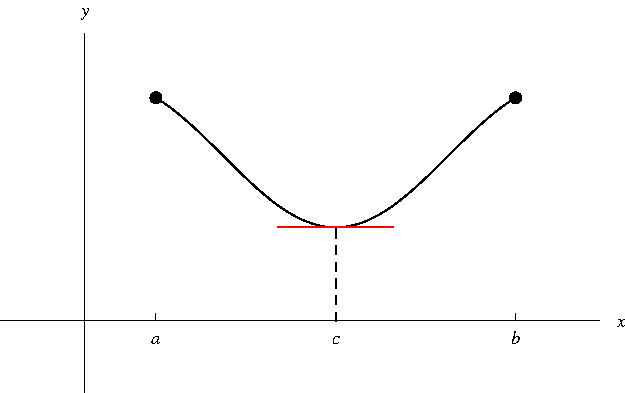
\includegraphics[height=2.5cm]{maxima-minima/pictures/04-02-rollesd.pdf}%
\column{.6\textwidth}
\begin{enumerate}
\setcounter{enumi}{2}
\item  $f(x) < f(a)$ for some $x$ in $(a,b)$.
\end{enumerate}
\begin{itemize}
\item<2->  By the Extreme Value Theorem, $f$ has a minimum in $[a,b]$.
\item<3->  Since $f(x) < f(a)$, this value is attained at some $c$ in $(a,b)$.
\item<4->  \alert<handout:0| 4>{Fermat's Theorem}: $f'(c) = 0$.\qedhere
\end{itemize}
\end{columns}
\end{proof}
\end{frame}
% end module rolles-theorem
